\chapter{Diseño e implementación} % Main chapter title

\label{Chapter3} % Change X to a consecutive number; for referencing this chapter elsewhere, use \ref{ChapterX}

\definecolor{mygreen}{rgb}{0,0.6,0}
\definecolor{mygray}{rgb}{0.5,0.5,0.5}
\definecolor{mymauve}{rgb}{0.58,0,0.82}

%%%%%%%%%%%%%%%%%%%%%%%%%%%%%%%%%%%%%%%%%%%%%%%%%%%%%%%%%%%%%%%%%%%%%%%%%%%%%
% parámetros para configurar el formato del código en los entornos lstlisting
%%%%%%%%%%%%%%%%%%%%%%%%%%%%%%%%%%%%%%%%%%%%%%%%%%%%%%%%%%%%%%%%%%%%%%%%%%%%%
\lstset{ %
  backgroundcolor=\color{white},   % choose the background color; you must add \usepackage{color} or \usepackage{xcolor}
  basicstyle=\footnotesize,        % the size of the fonts that are used for the code
  breakatwhitespace=false,         % sets if automatic breaks should only happen at whitespace
  breaklines=true,                 % sets automatic line breaking
  captionpos=b,                    % sets the caption-position to bottom
  commentstyle=\color{mygreen},    % comment style
  deletekeywords={...},            % if you want to delete keywords from the given language
  %escapeinside={\%*}{*)},          % if you want to add LaTeX within your code
  %extendedchars=true,              % lets you use non-ASCII characters; for 8-bits encodings only, does not work with UTF-8
  %frame=single,	                % adds a frame around the code
  keepspaces=true,                 % keeps spaces in text, useful for keeping indentation of code (possibly needs columns=flexible)
  keywordstyle=\color{blue},       % keyword style
  language=[ANSI]C,                % the language of the code
  %otherkeywords={*,...},           % if you want to add more keywords to the set
  numbers=left,                    % where to put the line-numbers; possible values are (none, left, right)
  numbersep=5pt,                   % how far the line-numbers are from the code
  numberstyle=\tiny\color{mygray}, % the style that is used for the line-numbers
  rulecolor=\color{black},         % if not set, the frame-color may be changed on line-breaks within not-black text (e.g. comments (green here))
  showspaces=false,                % show spaces everywhere adding particular underscores; it overrides 'showstringspaces'
  showstringspaces=false,          % underline spaces within strings only
  showtabs=false,                  % show tabs within strings adding particular underscores
  stepnumber=1,                    % the step between two line-numbers. If it's 1, each line will be numbered
  stringstyle=\color{mymauve},     % string literal style
  tabsize=2,	                   % sets default tabsize to 2 spaces
  title=\lstname,                  % show the filename of files included with \lstinputlisting; also try caption instead of title
  morecomment=[s]{/*}{*/}
}
%----------------------------------------------------------------------------------------

\textit{ NOTA: ESTE CAPÍTULO SE ENCUENTRA EN CONSTRUCCIÓN.}

En este capítulo se detallan los componentes de software y hardware diseñados e implementados por el autor, su interrelación, y los criterios seguidos.

%----------------------------------------------------------------------------------------
%	SECTION 1
%----------------------------------------------------------------------------------------
\section{Arquitectura del sistema}

Para abordar el trabajo realizado, en esta sección se expone la arquitectura general del sistema embebido implementado, esquematizada en el diagrama de la figura \ref{fig:diagramaCompleto}, y luego, en las siguientes secciones, se detallan cada uno de los componentes de manera individual.

\begin{figure}[htbp]
	\centering
	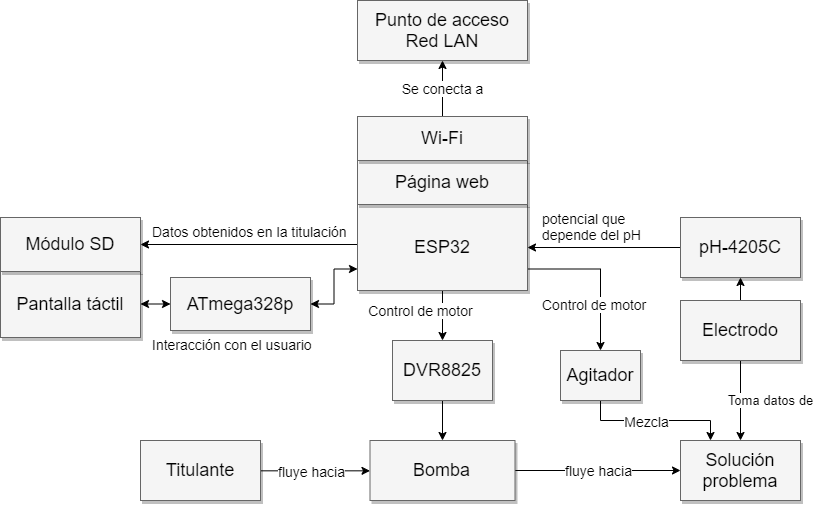
\includegraphics[width=1.0\textwidth]{./Figures/DiagramaBloquesCompleto.png}
	\caption{Diagrama en bloques del trabajo realizado.}
	\label{fig:diagramaCompleto}
\end{figure}

El componente principal del sistema es el ESP32, que tiene como función coordinar cada una de las partes intervinientes. A través de una comunicación del tipo UART, recibe las órdenes ingresadas a través de la pantalla táctil y  son procesadas por el ATmega328p, para realizar las configuraciones o funciones que solicite el usuario.

Dentro de las configuraciones, está la posibilidad de modificar el volumen de corte y de habilitar, o no, el agitador. El volumen de corte es la cantidad máxima de titulante que se utiliza durante la titulación. Cuando se alcanza ese valor, el proceso se detiene automáticamente. En cuanto a la habilitación del agitador, permite elegir si el mismo se activa o no al inicial la titulación.

Las funciones que ofrece el sistema son las de limpieza, calibración y titulación. El modo limpieza se utiliza para purgar la bomba previo al proceso de titulación y para eliminar los retos de titulante que quedan en las mangueras al finalizar el proceso. 

La calibración permite ajustar el valor leído por el ADC, en el cual se encuentra conectado el módulo pH4502C. Para llevarla a cabo, se hace uso de tres líquidos patrones, denominados \textit{buffers}, de pH 4, 7 y 10, respectivamente. Se debe realizar la calibración de manera periódica, ya que las propiedades del electrodo varían con el tiempo.

Una vez realizadas las configuraciones correspondientes, la limpieza y la calibración, es posible iniciar la titulación. Cuando esto sucede, el ESP activa  la bomba para que comience a inyectar el titulante en la muestra problema, y registra los valores de pH asociados, que obtiene desde el electrodo. En la pantalla se visualiza una curva del pH a lo largo del tiempo, y se ofrece la posibilidad de finalizar el proceso, mediante un botón, en el momento que el usuario lo desee. En caso contrario, el proceso finaliza al alcanzar el volumen de corte.

Una vez finalizado el proceso, el ESP32 calcula la derivada primera para cada valor de volumen y pH asociados, y, en base a ello, encuentra el valor de volumen inyectado en el punto final. Tanto este valor, como todos los valores registrados, se almacenan en la memoria SD, a través de una comunicación SPI con el módulo correspondiente, y en la página web, que se encuentra embebida en la memoria del ESP32. A través de una conexión de área local se puede acceder a esta página desde otro dispositivo y visualizar los resultados.

Para realizar las actividades mencionadas previamente, el ESP32 ejecuta tres tareas: la tarea encargada de la comunicación UART con el ATmega328p, que se aloja en el núcleo 0, y las tareas de medición del electrodo y de control de la bomba, que se alojan en el núcleo 1. Además, existe un controlador de eventos, que se ejecuta sobre el núcleo 0 cuando alguien accede a la página web.


%----------------------------------------------------------------------------------------
\section{Medición del electrodo}

La medición del electrodo es un módulo de software que tiene una tarea de FreeRTOS asociada. El objetivo de esta tarea es obtener el valor en mV que entrega el módulo pH-4502C y es ejecutada durante el proceso de calibración y el de titulación. En el código \ref{cod:tareaElectrodo} se muestra el pseudocódigo de la tarea de medición del electrodo. Al inicio de esta tarea se realiza la configuración del ADC utilizado, el cual se habilita con resolución 12 bits en el pin correspondiente al canal 6 del ADC número 1.

La lectura del valor del ADC se acumula en la variable sumaAdc durante las N iteraciones del bucle for. Cada una de estas iteraciones se realiza en un intervalo de 10 mS, y, al finalizar el bucle for, el valor total se divide por la cantidad de muestras realizadas, lo que permite promediar el valor leído y así reducir el ruido presente en la conversión, tal y como sugiere la página oficial del ESP32 \citep{WEBSITE:2}. Cabe destacar que el acceso a la variable valorAdc está protegido por una sección crítica, ya que resto de las tareas también pueden acceder a la variable cuando precisan calcular el valor de pH.

\begin{lstlisting}[label=cod:vControl,caption=Pseudocódigo de la tarea de medición de pH.]
void tareaElectrodo (void *arg)
{
    //Configuracion de resolucion y pin del ADC
    configuracionADC(12 bits, pin);
    uint32_t sumaAdc = 0;

    while(true)
    {
    for (int i=0; i< N_MUESTRAS; i++)
    {
        sumaAdc = sumaAdc + lecturaADC(pin);  
        vTaskDelay(10 mS);
    } 
    inicioSeccionCritica(); 
    valorAdc = sumaAdc / N_MUESTRAS;
    finSeccionCritica();
    sumaAdc = 0;
    }
}
	\label{cod:tareaElectrodo}
\end{lstlisting}

%----------------------------------------------------------------------------------------
\section{Control de la bomba}

En la figura \ref{fig:flujoBomba} se muestra el diagrama de flujo de la tarea de control de la bomba.

\begin{figure}[htbp]
	\centering
	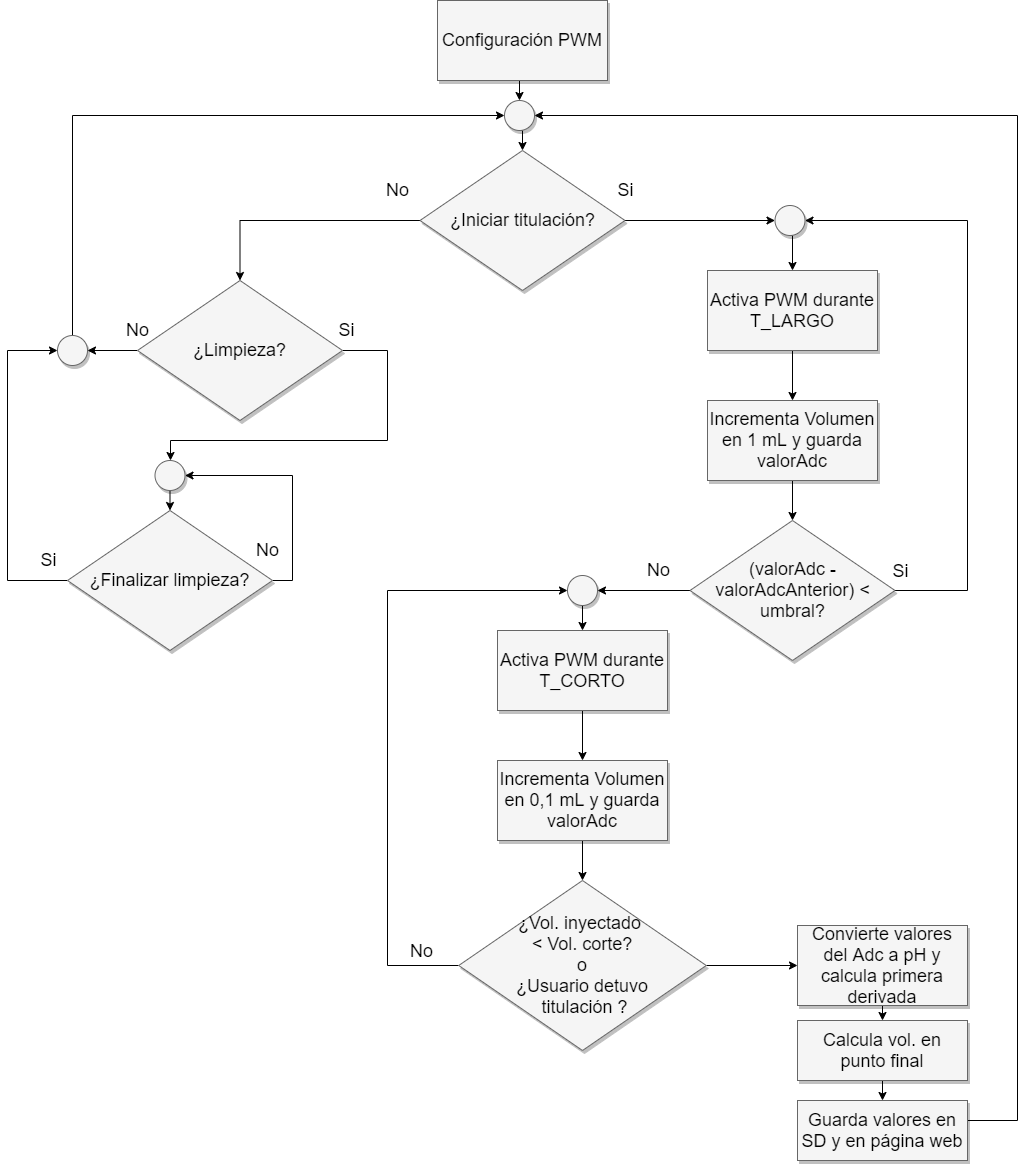
\includegraphics[width=1.0\textwidth]{./Figures/motorBomba.png}
	\caption{Diagrama de flujo de la tarea de control de la bomba.}
	\label{fig:flujoBomba}
\end{figure}


%----------------------------------------------------------------------------------------
\section{Interfaz de usuario}

%----------------------------------------------------------------------------------------
\section{Almacenamiento de datos}

%----------------------------------------------------------------------------------------
\section{Servidor web}

%----------------------------------------------------------------------------------------
\section{Esquemáticos y PCB}
